\documentclass[a4paper]{article}
\usepackage[utf8x]{inputenc}
\usepackage[T1,T2A]{fontenc}
\usepackage[russian]{babel}
\usepackage{hyperref}
\usepackage{indentfirst} % включить отступ у первого абзаца
\usepackage{listings}
\usepackage{color}
\usepackage{here}
\usepackage{graphicx}
\usepackage{caption}
\lstset{ %
language=bash,                % choose the language of the code
basicstyle=\footnotesize,       % the size of the fonts that are used for the code
numbers=left,                   % where to put the line-numbers
numberstyle=\footnotesize,      % the size of the fonts that are used for the line-numbers
stepnumber=1,                   % the step between two line-numbers. If it is 1 each line will be numbered
numbersep=5pt,                  % how far the line-numbers are from the code
backgroundcolor=\color{white},  % choose the background color. You must add \usepackage{color}
showspaces=false,               % show spaces adding particular underscores
showstringspaces=false,         % underline spaces within strings
showtabs=false,                 % show tabs within strings adding particular underscores
frame=single,           % adds a frame around the code
tabsize=2,          % sets default tabsize to 2 spaces
captionpos=b,           % sets the caption-position to bottom
breaklines=true,        % sets automatic line breaking
breakatwhitespace=false,    % sets if automatic breaks should only happen at whitespace
escapeinside={\%*}{*)},          % if you want to add a comment within your code
postbreak=\raisebox{0ex}[0ex][0ex]{\ensuremath{\color{red}\hookrightarrow\space}}
}

\usepackage[left=2.5cm, top=2cm, right=2cm, bottom=2cm, nohead]{geometry}

\begin{document}
\begin{titlepage}

\begin{center}

\large Санкт-Петербургский Политехнический Университет Петра Великого\\
\large Институт компьютерных наук и технологий \\
\large Кафедра компьютерных систем и программных технологий\\[6cm]

\huge Сети ЭВМ и телекоммуникации\\[0.5cm]
\large Отчет по лабораторной работе\\[5cm]
\end{center}

\begin{flushright}
\begin{minipage}{0.5\textwidth}
\begin{flushright}
\textbf{Работу выполнил:}

Петров В.Д.

{Группа:} 43501/4\\


\textbf{Преподаватель:} 

Зозуля А.В.
\end{flushright}
\end{minipage} % конец врезки
\end{flushright} % конец выравнивания по левому краю

\vfill % заполнить всё доступное ниже пространство

\begin{center}

\large Санкт-Петербург\\
\large \the\year % вывести дату

\end{center} % закончить выравнивание по центру

\thispagestyle{empty} % не нумеровать страницу
\end{titlepage} % конец титульной страницы

\vfill % заполнить всё доступное ниже пространство

\section{Цель работы}
\begin{itemize}
\item Приобретение базовых навыков работы с сокетами;
\item Изучение библиотек BSD-socket и WinSock;
\item Изучение возможностей протоколов TCP и UDP;
\item Изучение принципов организации клиент-серверных приложений.
\end{itemize}
\section{Базоыве работы}
\subsection{Простейшие TCP сервер и клиент}
\begin{figure}[H]
\begin{center}
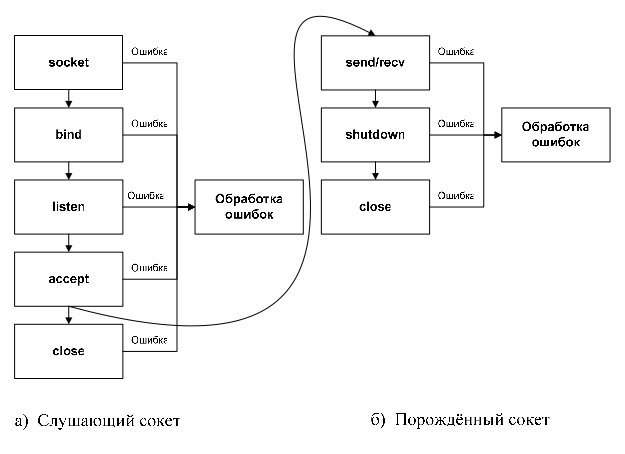
\includegraphics[scale=0.7]{pics/ttcps.png}
\caption{Структура типичного TCP-сервера}
\label{pic:ttcps}
\end{center}
\end{figure}
\begin{center}
\textbf{int} socket( \textbf{int} domain, \textbf{int} type, \textbf{int} protocol );
\end{center}

Параметр в качестве параметра domain передаем AF\_INET, то есть сокет создается для передачи с использованием TCP/UDP. Параметр type определяет тип создаваемого сокета. Для использования протокола TCP требуется передать SOCK\_STREAM. Параметр protocol зададим равным 0, так как в данном случае протокол определяется типом создаваемого сокета. Для сервера обязательно привязать сокет к определенному IP-адресу и порту, чтобы клиенты знали его и могли к нему подключиться. Для этого осуществляется вызов bind(). После этого сокет переводится в режим прослушивания, для чего используется вызов listen(). Теперь этот сокет будет ожидать входящего соединения. Для того, чтобы принять соединение выполняется вызов accept(). Она возвращает дескриптор сокета, соединенного с клиентом. Они имеет точно такой же адрес и порт, как и слушающий сокет. Слушающий сокет при этом остаётся в режиме прослушивания. Заметим, что существование сокетов с одинаковыми параметрами возможно, потому что уникальным должно быть соединение (пара скоетов), а не сокет. Теперь можно осуществлять обмен данными, используя только что созданный сокет. Для передачи и приема данных используются вызовы send() и recv(). После окончания обмена соединение необходимо корректно завершить. Для этих целей используются вызовы shutdown()  и close(). Отметим, что в ОС Windows  можно не вызывать shutdown, а вот в Linux этот вызов необходим. После этого можно закрывать слушающий сокет.
\begin{figure}[H]
\begin{center}
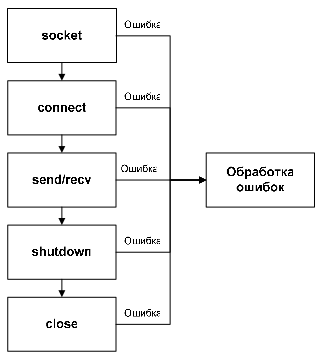
\includegraphics[scale=0.7]{pics/ttcpc.png}
\caption{Структура типичного TCP-клиента}
\label{pic:ttcpc}
\end{center}
\end{figure}
Как видно, структура клиента проще. Адрес и порт клиента могут быть любыми из доступных, поэтому не требуется вызывать bind(). Для подключения к серверу нужно установить соединение с помощью вызова connect(). После этого можно обмениваться данными.
	
Итак, при таком подходе можно реализовать простейший эхо-сервер с возможностью подключения одного клиента. Но сервер должен уметь обслуживать множество клиентов одновременно, поэтому любой сервер обязательно поддерживает многопоточность.
\subsection{Многопоточный TCP сервер}
\begin{figure}[H]
\begin{center}
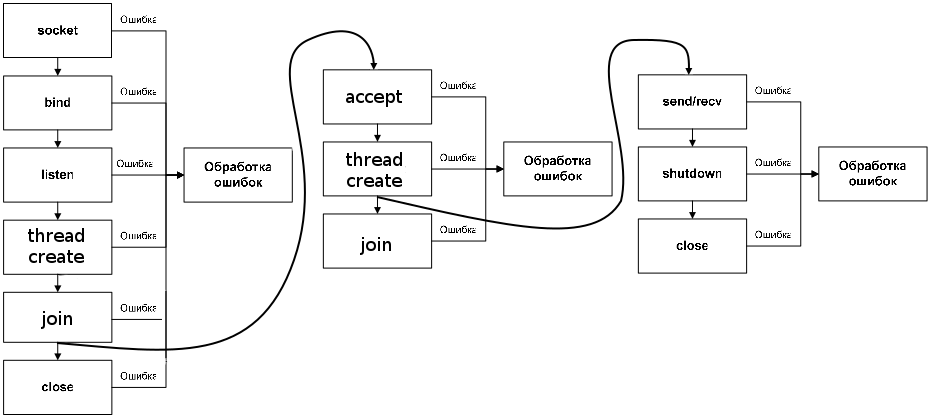
\includegraphics[scale=0.5]{pics/mtcps.png}
\caption{Структура многопоточного TCP-сервера}
\label{pic:mtcps}
\end{center}
\end{figure}
В основном потоке осуществляется создание сокета, привязка к  адресу и порту, перевод в режим прослушивания. После чего запускается поток, в котором циклически выполняется accept(). Теперь поток «свободен» и в нем можно осуществлять взаимодействие с пользователем.
В accept-потоке осуществляется прием соединения и выделение сокета для взаимодействия с подключившимся клиентом. После чего создается отдельный клиентский поток, в котором и производится обмен данными. Таких потоков может быть много.

Имеет смысл хранить дескрипторы всех созданных сокетов. Это позволяет закрыть сокет в любом месте программы, где имеется доступ к массиву дескрипторов, что приведет к возникновению ошибки при выполнении вызовов send/recv/accept. В этом случае управление должно быть передано в блок завершения потока. Таким образом, потоки завершатся сами, что является наиболее предпочтительным путем завершения потоков. Кроме того, для корректного завершения потоков и освобождения ресурсов требуется, чтобы те потоки, которые имеют дочерние потоки, дождались их завершения.

При разработке многопоточных приложении следует особенно внимательно отнестись к использованию глобальных ресурсов (например, переменных). Для корректной работы приложения необходимо, чтобы в каждый момент времени доступ к конкретному ресурсу был только у одного потока. Нужно решать проблему синхронизации потоков. Для этого существует множество средств. Конкретно в данной работе использовались мьютексы.

Мьютексы — специальные объекты ядра, использующиеся для защиты объектов от доступа к ним других потоков. Поток, которому требуется выполнить операции с объектом, захватывает охраняющий его мьютекс. Теперь доступ к объекту имеется только у него, а остальные потоки вынуждены ждать, пока освободится мьютекс. После того, как требуемые действия будут выполнены, поток должен освободить мьютекс, чтобы объектом могли воспользоваться другие потоки. 

В нашем примере глобальным ресурсом (объектом) может быть массив дескрипторов сокетов. Операция добавления элемента в массив выполняется в accept-потоке, а удаление из массива происходит перед "схлопованием" потока. Следовательно, массив дескрипторов следует защитить мьютексом. Кроме того, данные самой программы(новости и темы) доступны из разных потоков, поэтому их тоже необходимо защитить.
\subsection{Простейшие UDP сервер и клиент}
\begin{figure}[H]
\begin{center}
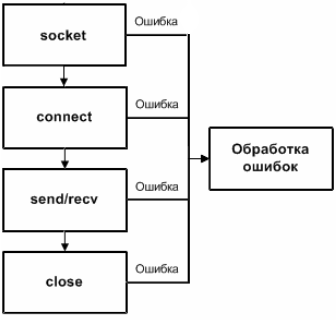
\includegraphics[scale=0.5]{pics/tudpc.png}
\caption{Структура простейшего UDP-клиента}
\label{pic:tudpc}
\end{center}
\end{figure}

При использовании протокола UDP соединение не устанавливается, следовательно, требуется осуществлять привязку сокета клиента к адресу и порту. Вызов connect() для протокола UDP задает адрес по умолчанию. Это позволяет использовать функции send() и recv(). При этом прием пакетов осуществляется только с этого адреса. Если вызов connect() не используется, то обмен осуществляется с помощью функций recvfrom() и sendto(), которые содержат дополнительные параметры, через которые передается адрес.

\begin{figure}[H]
\begin{center}
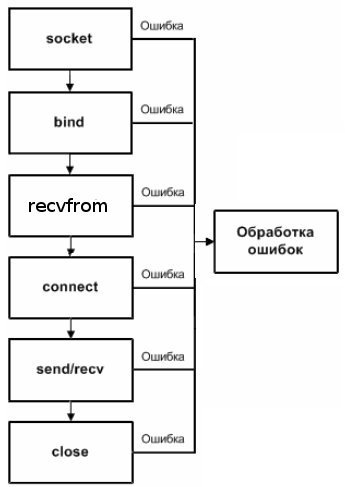
\includegraphics[scale=0.5]{pics/tudps.png}
\caption{Структура простейшего UDP-сервера}
\label{pic:tudps}
\end{center}
\end{figure}

Для применения фкнкции connect(), необходимо знать, к какому адресу и порту производить привязку. Для этого используется recvfrom(), принимающая первый пакет. Она позволяет узнать, автора пакета и к нему применить connect().

\section{Индивидуальное задание}
\noindent Номер задания: \textbf{1.2.13}\\
Тема задания: \textbf{Система поиска/публикации новостей}\\[1cm]

Задание требует разработать приложение–клиент и приложение–сервер системы поиска/публикации новостей. Новости сгруппированы по темам. Каждая новость имеет уникальный идентификатор, название и текст новости.

\textbf{Основные возможности}. Серверное приложение должно реализовывать следующие функции:
\begin{itemize}
\item Прослушивание определенного порта
\item Обработка запросов на подключение по этому порту от клиентов
системы поиска/публикации новостей
\item Поддержка одновременной работы нескольких клиентов системы
поиска/публикации новостей через механизм нитей
\item Прием запросов от клиента на передачу списка тем, списка новостей
по теме, текста новости, добавление новости по теме
\item Осуществление добавления тем, новостей по темам
\item Передача списков тем, списков новостей и текстов новостей
\item Обработка запроса на отключение клиента
\item Принудительное отключение клиента
\end{itemize}

Клиентское приложение должно реализовывать следующие функции:
\begin{itemize}
\item Установление соединения с сервером
\item Передача запросов на передачу списка тем, списка новостей по теме,
текста новости, добавление новости по теме
\item Получение результатов от сервера
\item Разрыв соединения
\item Обработка ситуации отключения клиента сервером
\end{itemize}

\textbf{Настройки приложений.}

Разработанное клиентское приложение должно предоставлять пользователю настройку IP–адреса или доменного имени сервера системы поиска/публикации новостей и номера порта, используемого сервером.

\textbf{Методика тестирования.}

Для тестирования приложений запускается
сервер системы поиска/публикации новостей и несколько клиентов. В процессе тестирования проверяются основные возможности приложений попередаче и приему сообщений.
\subsection{Протокол для TCP}
Структура приложения остаётся схожей с приведённой на рис. \ref{pic:mtcps}. Меняется только работа с передаваемыми сообщениями.
\begin{table}[H]
\begin{center}
\caption{Система команд протокола для обмена с использованием TCP}
\label{tabular:TCPstruct}
\begin{tabular}{|l|l|}
\hline
LIST & запрос списка тем\\ \hline
LIST <theme> & запрос спска новостей в данной теме\\ \hline
LEN <number of lines> & предупреждение о количестве строк\\ \hline
ADDN <theme> <text> & добавление новости в тему\\ \hline
SHOW <pon id> & запрос новости\\ \hline
HELP & запрос списка команд, поддерживаемых сервером\\ \hline
\end{tabular}
\end{center}
\end{table}

Все ответы сервера клиенту является текстом, кроме предупреждения о длине. Ошибки не были вынесы в отдельный формат пакета. Это можно было бы реализовать двумя путями: добавлением соответствующей метки в пакета с текстом или формат пакета ошибки с кодом. Второй вариант требует знания всех возможных ошибок от сервера, но уменьшает траффик.

Получается, в данной вариации протокол описывает сообщения от клиента к серверу (таб. \ref{tabular:TCPstruct}) и одно сообщение от сервера (LEN). Это сообщение предупреждает о количестве строк, в ответе
Функцианальность добавления тем не внесена в протокол, так как данные хранятся на сервере, а операция доступна только серверу. Так что по сети подобные запросы не передаются.
\subsection{Протокол для UDP}
Для удобства структура приложения была сохранена. Для этого поток, ответственный за accept() был заменён на поток, создающий новые UDP сокеты и переводящий дальшейшее общение с клиентом на них. Для этого были добавлены дополнительные пакеты приветствия - HEL. С помошью такого пакета клиент в начале общения сообщает серверу свои адрес и порт, а сервер в ответ таким же пакетом сообщает параметры нового сокета, выделенного для данного клиента.

Завершение общения сопровождается посылкой пакета BEY.

А необходимость сообщать количество строк отпала, так как нет потока, из которого нужно выделять пакеты.
\begin{table}[H]
\begin{center}
\caption{Система команд протокола для обмена с использованием UDP}
\label{tabular:UDPstruct}
\begin{tabular}{|l|l|}
\hline
LIST & запрос списка тем\\ \hline
LIST <theme> & запрос спска новостей в данной теме\\ \hline
ADDN <theme> <text> & добавление новости в тему\\ \hline
SHOW <pon id> & запрос новости\\ \hline
HELP & запрос списка команд, поддерживаемых сервером\\ \hline
HEL & Представление серверу или клиенту\\ \hline
BEY & Предупреждение о завершение связи\\ \hline
\end{tabular}
\end{center}
\end{table}
\subsection{Тестирование}
Проверка одновременного обслуживания нескольких клиентов проводилась путем запуска нескольких клиентов и выполнения ими предусмотренных действий.

Так как вся сетевая надёжность в TCP реализации ложится на TCP нареканий в работе обнаружено не было.

UDP реализация была подвергнута большему количесву испытаний. Так через loopback была провера работа в условиях "идельной" сети. 

Потеря пакетов отсутствовала и приложения работали корректно. Однако, всвязи с особенностями реализации сервера, принудительное отключение клиента от сервера не происходило мгновенно, так как закрытие сокето не приводело к немедленному закрытию потока, но не позволяло продолжить общение с клиентом. Функция select() ждала сообщения от клиента и не реагировала на выключение и закрытие сокета. Но по истечению таймера, ресурсы освобождались.

Вопрос о порядке передачи отсутствует, так как избегается ситуация деления сообщения на несколько дэйтограм. Но в тако случе помогло бы сообщение, сообщающее об общем количесве и нумерация последующих.

При ухужшение параметров сети (задержка и потери) с помощью средств встроенных в ядро ОС Linux tc и netem были получены завершение клиента(ответ от вервера не успевал прийти за 4 секнды, отведённые на ожидание) и закрытие потока клиента (не приходили сообщения от него в течение 10 минут).

Так как нашей задачей не являлась абсолютная надёжность, я был удолетворён информированием о проблеме без её решения, поэтому дополнительные пакеты подтверждения отсутствуют, как и хранение и повторная посылка потерянных пакетов.

Тестирование на утечки памяти с помощью valgrind в ручном режиме задания маршрута утечек не выявило.
\section{ Вывод}
Протоколы TCP и UDP используются для разных целей. Если требуется вести диалог между сервером и клиентом, предпочтительней использовать TCP. Если же общение ограничивается запросом – ответом, можно обойтись UDP-протоколом.

Протокол TCP удобней в программировании, так как сам по себе обеспечивают большую надежность, чем UDP, которую в последнем требуется обеспечить самому программисту. Разумеется, протокол UDP работает гораздо быстрее, и если приложению скорость передачи данных важнее надёжности, то нужно использовать именно его.
 
Таким образом,  требуемая надежность протокола и скорость передачи данных являются факторами, определяющими выбор того или иного протокола. В случае инвидидуального задания, требуется тадёжность передачи, а скорость маловажна, поэтому разумно выбрать для такого приложения TCPю

Реализуемый прикладной протокол не является универсальным. Чтобы его можно было использовать и с TCP, и с UDP, требуется вносить изменения. Так в UDP требуется обеспечивать надёжность на прикладном уровне, а в TCP выделять из потока пакеты.
\newpage
\section{Приложения}
\captionof{lstlisting}{тривиальный TCP-клиент}
\lstinputlisting{../TrivialTCP/Client/main.c}

\captionof{lstlisting}{тривиальный TCP-сервер}
\lstinputlisting{../TrivialTCP/Server/main.c}

\captionof{lstlisting}{многопоточный TCP-сервер}
\lstinputlisting{../TrivialTCP/ServerMT/main.c}

\captionof{lstlisting}{тривиальный UDP-клиент}
\lstinputlisting{../TrivialUDP/client.c}

\captionof{lstlisting}{тривиальный UDP-сервер}
\lstinputlisting{../TrivialUDP/server.c}

\captionof{lstlisting}{TCP-клиент}
\lstinputlisting{../TCP/client.c}

\captionof{lstlisting}{TCP-сервер}
\lstinputlisting{../TCP/server.c}

\captionof{lstlisting}{UDP-клиент}
\lstinputlisting{../UDP/client.c}

\captionof{lstlisting}{UDP-сервер}
\lstinputlisting{../UDP/server.c}
\end{document}